\documentclass[]{article}

\usepackage[english]{babel}
\usepackage{graphicx}
\usepackage{booktabs}
\usepackage{float}
\usepackage{hyperref}

\title{Wind Prediction with LSTM}
\author{Juan Lao Tebar}

\begin{document}
	
\maketitle

\begin{abstract}
	
LSTM neural networks are powerful learning models, specially on long sequences with relations in long intervals of time. In this practice we analyze their behavior against the WIND dataset, implementing several Deep Learning techniques to improve the learning process and to prevent overfitting.
	
\end{abstract}

\section{Introduction}

In this practice we extend the experiments performed in the previous ``Guided Laboratory of the RNN Topic''\footnote{https://upc-mai-dl.github.io/rnn-lab-guided/}, not only predicting more steps and trying more complex topologies, but also testing different ways of preparing the data to exploit the true power of LSTM networks, learning the inherent data relations over long intervals of time.

As explained in the guided laboratory, the data for this example is a subset of the NREL Wind Integration National Dataset (WIND) Toolkit\footnote{https://www.nrel.gov/grid/wind-toolkit.html}. The original set consists of meteorological information for more than 126,000 sites across the USA from 2007 to 2013, sampled every 5 minutes. However, for our purposes, we only take into account the data from one site sampled every 15 minutes.

In the guided laboratory we took into account only one variable---wind speed at 100m---and we predicted the value it takes in the following step. In contrast, in this practice we predict the following 6 steps including the rest of the variables: air density, temperature and air pressure.

The workflow of this practice consists in defining a baseline model---similar to the one proposed in the guided laboratory---and improving it in the following experiments, step by step.

More in detail, the plan consists in the following:

\begin{enumerate}
	\item Study the effect of incrementing the number of hidden layers.
	\item Observe the response of the model for different activation functions.
	\item Find a better window size.
	\item If the model overfits the training data, apply dropout---on inter-layer connections and/or on LSTM gates.
	\item In case of experimenting explosive gradients, avoid them with gradient clipping.
	\item Present a new sequence-to-sequence model capable of learning from \emph{any-length} input samples.
\end{enumerate}

The code related to this work is public and available at github\footnote{https://github.com/juanlao7/WIND-LSTM}.

\section{Experiments}

The original data set consists of 245,472 measurements. In our process we use 122,736 of them for training---$\sim$3.5 years---, 61,368 for validation and 61,368 for testing---$\sim$1.75 years.

The loss of the model is measured with the mean squared error (MSE).

\subsection{Baseline}

Our first model is quite similar to the one proposed in the previous guided laboratory, as it consists of an LSTM layer of 512 units connected to a dense output layer of 24 units---6 predictions of 4 variables---, as it can be seen in figure \ref{f:model}. We use ReLU as the activation function of the LSTM units, the logistic function for their recurrent step and, of course, a linear function for the output neurons.

\begin{figure}[H]
	\centering
	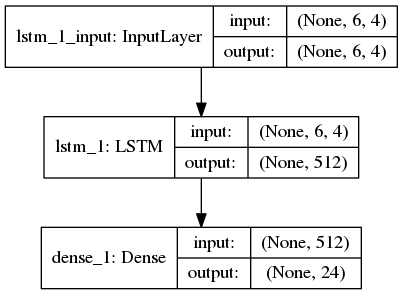
\includegraphics[width=0.5\textwidth]{model}
	\caption{Structure of the baseline model.}
	\label{f:model}
\end{figure}

We train the model in batches of 1000 samples using the adaptive optimizer RMSprop \cite{tieleman2012lecture}---recommended for training recurrent neural networks---with a learning rate of 0.0001, $ \rho = 0.9 $, $ \varepsilon = 1 \cdot 10^{-8} $ and no learning rate decay. The samples are obtained by \emph{lagging} the original samples of the data set with their previous 6 steps and foreseeing the following 6.

In this practice we change the stopping criteria of the training process, as we remove the limit of epochs and we implement a stopper based on the validation loss: when we detect a minimum value, we stop the training after 30 epochs if it does not decrease.

With this configuration we obtain the results shown in table \ref{t:baseline}.

\begin{table}[H]
	\centering
	\begin{tabular}{@{}ccc@{}}
		\toprule
		Training loss & Validation loss & Test loss \\ \midrule
		0.02878       & 0.03151         & 0.03290   \\ \bottomrule
	\end{tabular}
	\caption{Results of the baseline model.}
	\label{t:baseline}
\end{table}

\subsection{Number of Layers}

Feedforward neural networks with two hidden layers can represent any decision boundary with arbitrary accuracy using the proper number of units, as well as approximating any smooth variable relation to any accuracy too.

For this reason, in this experiment we compare our previous results with the ones obtained with models of two and three hidden LSTM layers of 512 units each.

Table \ref{t:layers} shows the results obtained, while figure \ref{f:layers} shows the evolution of the training and validation loss in each case.

\begin{table}[H]
	\centering
	\begin{tabular}{@{}cccc@{}}
		\toprule
		& Training loss & Validation loss & Test loss \\ \midrule
		1 hidden layer  & 0.02878       & 0.03151         & 0.03290   \\
		2 hidden layers & 0.02771       & 0.03088         & 0.03257   \\
		3 hidden layers & 0.02830       & 0.03207         & 0.03327   \\ \bottomrule
	\end{tabular}
	\caption{Results after testing different number of hidden layers.}
	\label{t:layers}
\end{table}

\begin{figure}[H]
	\centering
	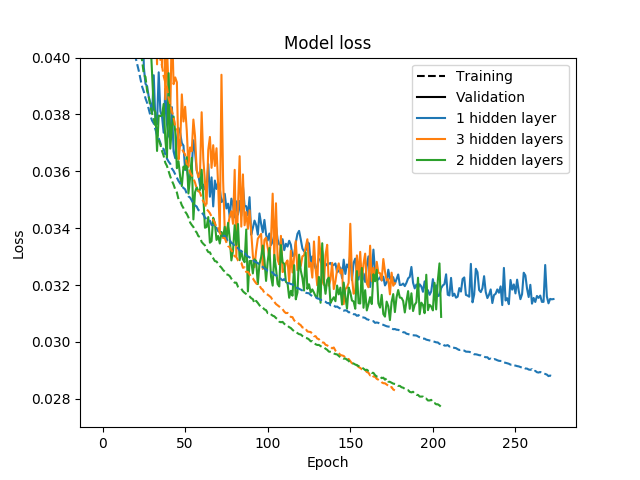
\includegraphics[width=0.5\textwidth]{layers}
	\caption{Validation and training loss with each number of hidden layers.}
	\label{f:layers}
\end{figure}

As expected, two hidden layers approximate better our data relations, while three hidden layers does not seem to improve the mark. In the following experiments we use an architecture of two hidden LSTM layers.

\subsection{Activation Function}

Clevert, Unterthiner, \& Hochreiter, 2016 \cite{clevert2015fast} found that using ELU instead of ReLU not only speeds up the learning process in deep neural networks, but also leads to higher classification accuracies: ``In contrast to ReLUs, ELUs have negative values which allows them to push mean unit activations closer to zero like batch normalization but with lower computational complexity. Mean shifts toward zero speed up learning by bringing the normal gradient closer to the unit natural gradient because of a reduced bias shift effect''.

In this experiment we aim to reproduce similar results, testing different activation functions---softplus, logistic, hyperbolic tangent, ELU and ReLU---for the hidden LSTM layers of our model, but still using the logistic function for their recurrent step.

Table \ref{t:activation} shows the results obtained, while figure \ref{f:activation} shows the evolution of the training and validation loss in each case.

\begin{table}[H]
	\centering
	\begin{tabular}{@{}ccccc@{}}
		\toprule
		& Training loss & Validation loss & Test loss & Epochs \\ \midrule
		Softplus           & 0.02972       & 0.03352         & 0.03485   & 288    \\
		Logistic           & 0.02986       & 0.03217         & 0.03348   & 622    \\
		Hyperbolic tangent & 0.02864       & 0.03133         & 0.03289   & 172    \\
		ELU                & 0.02856       & 0.03143         & 0.03251   & 186    \\
		ReLU               & 0.02771       & 0.03088         & 0.03257   & 206    \\ \bottomrule
	\end{tabular}
	\caption{Results after testing different activation functions.}
	\label{t:activation}
\end{table}

\begin{figure}[H]
	\centering
	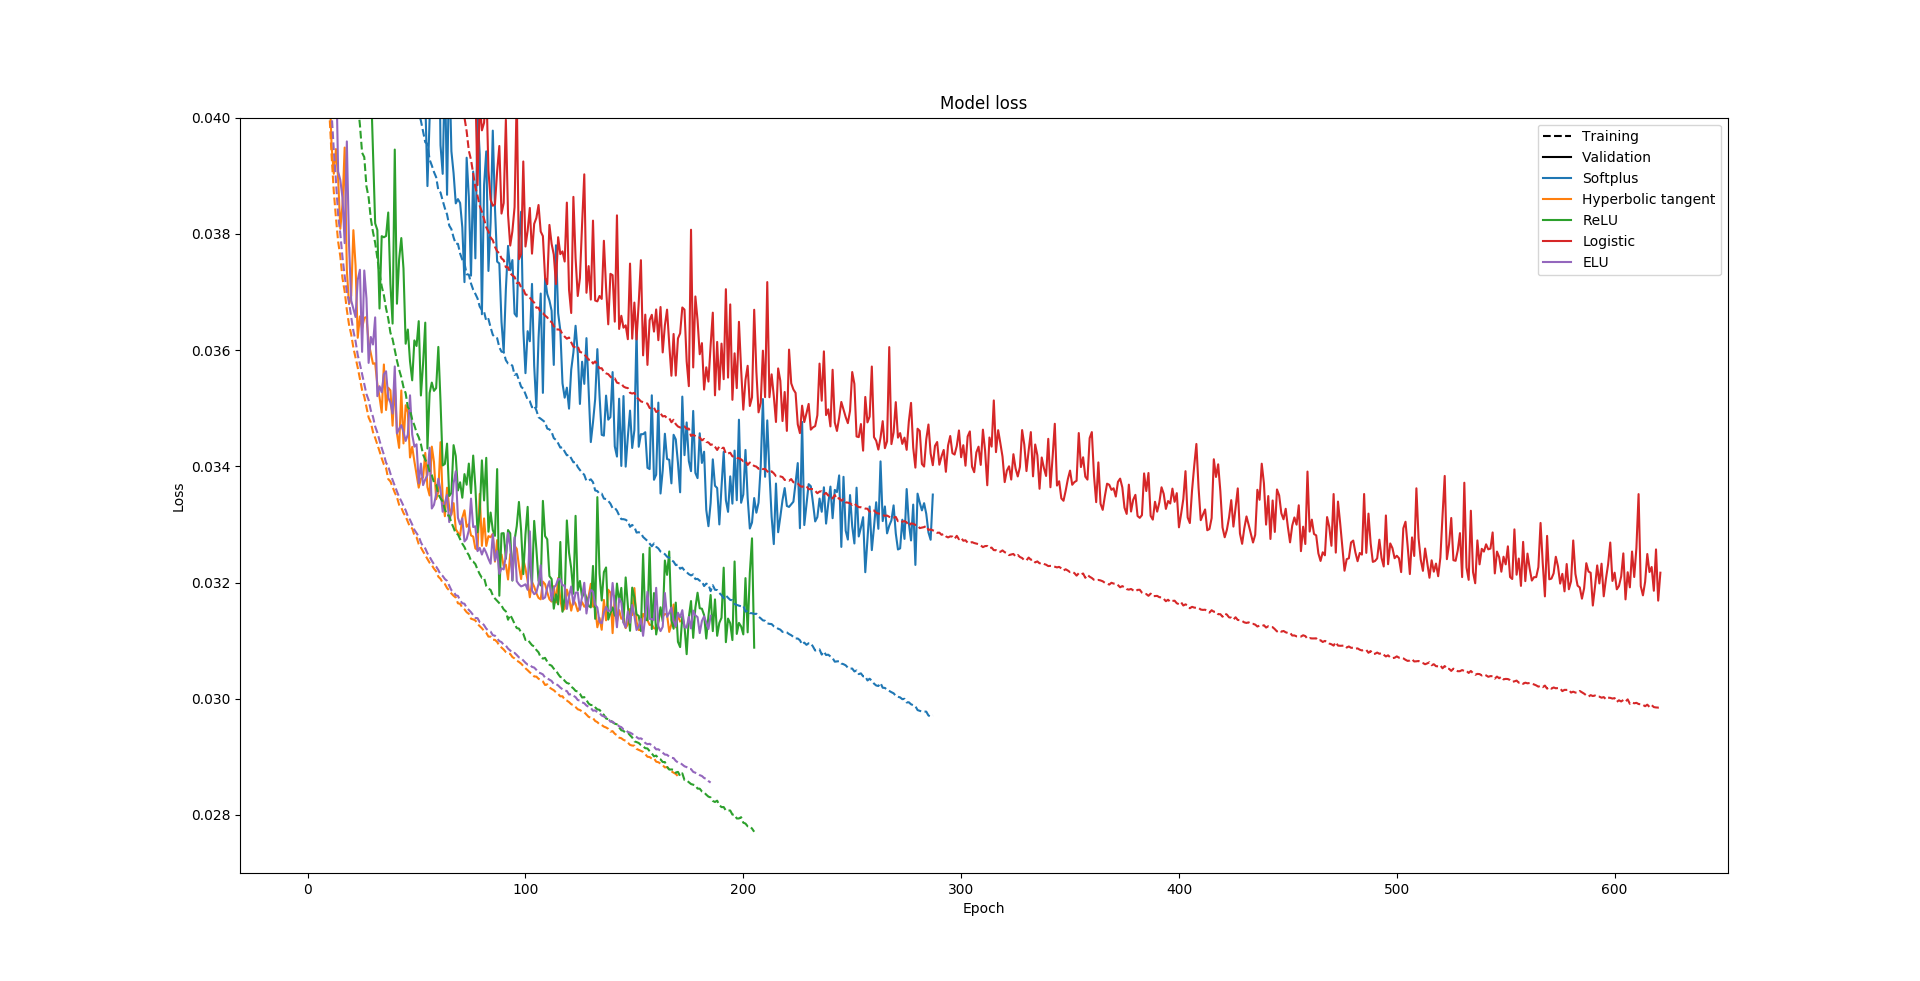
\includegraphics[width=\textwidth]{activation}
	\caption{Validation and training loss with each activation function.}
	\label{f:activation}
\end{figure}

As we can see, in our case ELUs and ReLUs are quite similar. We can see how ELUs take a slightly lesser number of epochs to converge, with almost the same test loss as with ReLUs but with higher training and validation losses.

In the following experiments we keep ReLU as the activation function for all the units of the hidden layers, since it is computationally cheap and we have not seen any considerable improvement on using ELU.

\subsection{Window Size}

Our data set is generated by going through the original samples with a window size of 12---6 measurements for the input + 6 for the output---. We must note that these measurements have been taken in intervals of 15 minutes, hence each input vector of the generated data set comprises an interval of 75 minutes.

In this experiment we test different window sizes, in order to determine if larger time intervals provide useful information for our model to obtain a lower loss.

Table \ref{t:window} shows the results obtained, while figure \ref{f:window} shows the evolution of the training and validation loss in each case.

\begin{table}[H]
	\centering
	\begin{tabular}{@{}cccc@{}}
		\toprule
		& Training loss & Validation loss & Test loss \\ \midrule
		Input size of 1  & 0.03595       & 0.03743         & 0.03810   \\
		Input size of 6  & 0.02771       & 0.03088         & 0.03257   \\
		Input size of 12 & 0.02655       & 0.03190         & 0.03345   \\
		Input size of 24 & 0.02242       & 0.03655         & 0.03743   \\
		Input size of 48 & 0.01975       & 0.04247         & 0.04327   \\ \bottomrule
	\end{tabular}
	\caption{Results after testing different window sizes.}
	\label{t:window}
\end{table}

\begin{figure}[H]
	\centering
	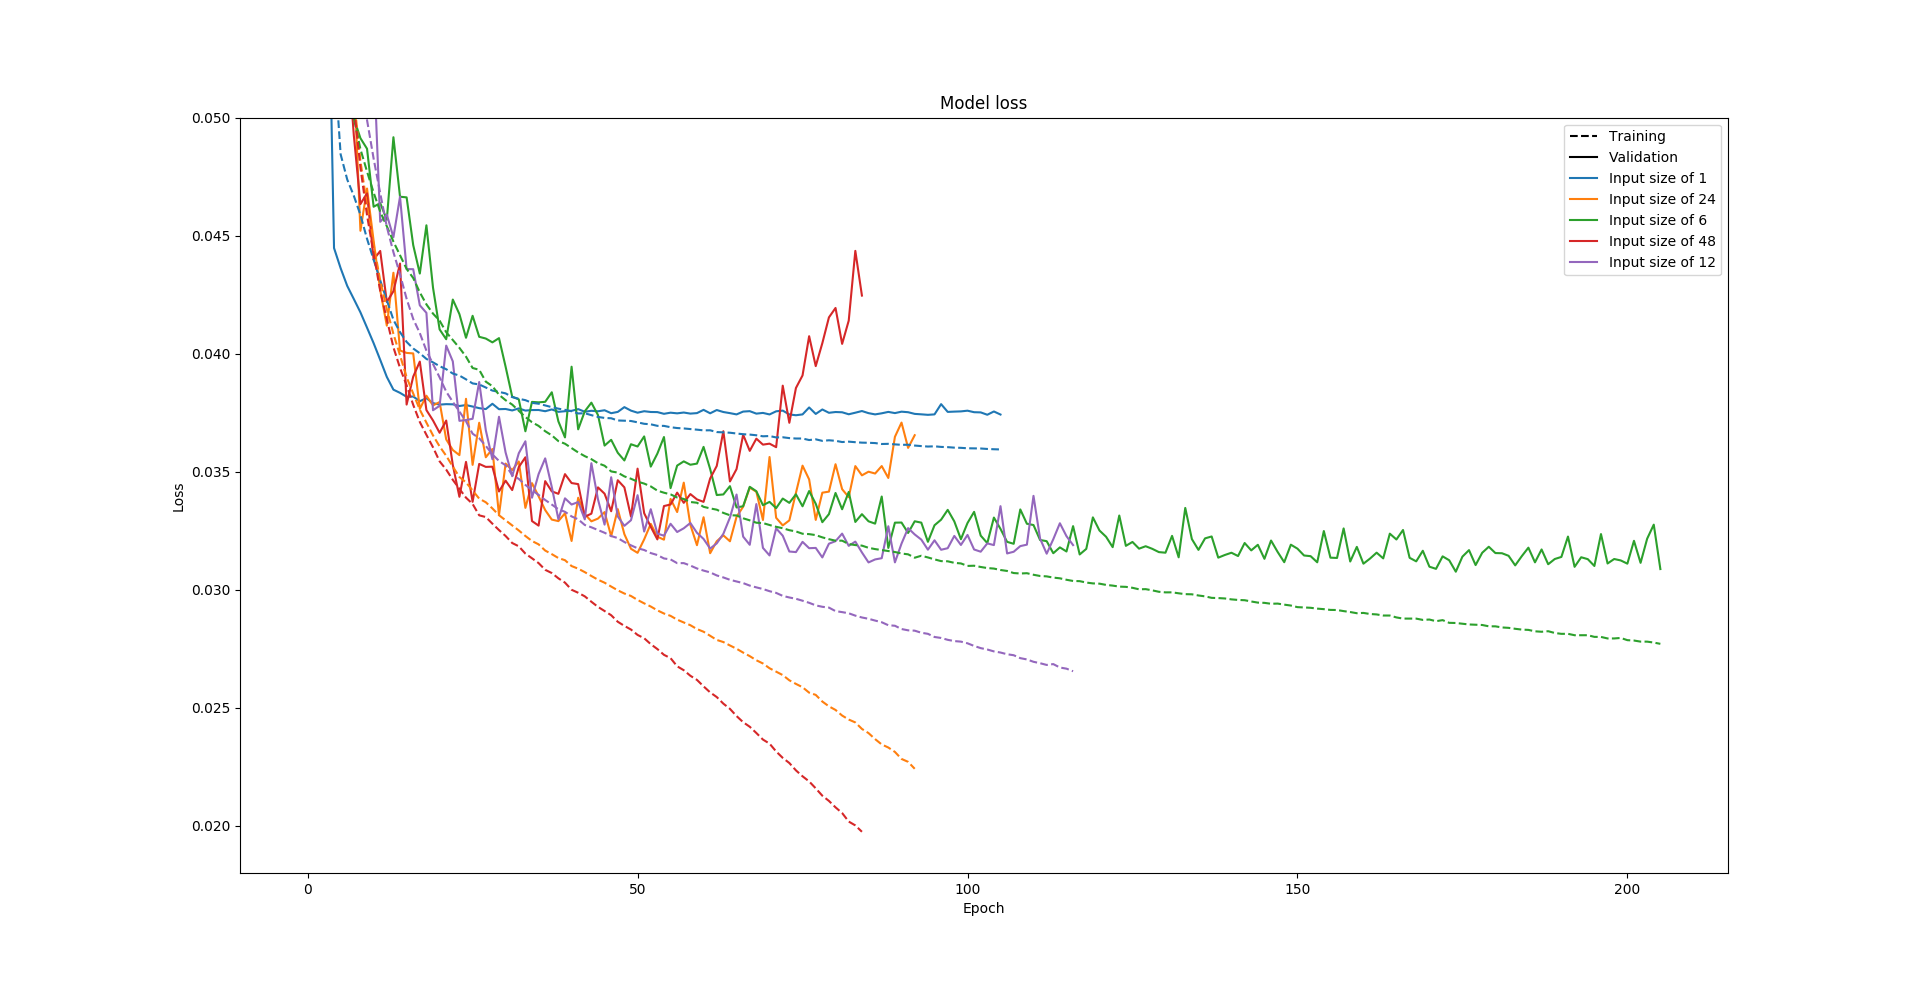
\includegraphics[width=\textwidth]{window}
	\caption{Validation and training loss with each window size.}
	\label{f:window}
\end{figure}

In this experiment we test input sizes up to 48. When we test higher values, at some point our gradients explode, loss becomes $ +\infty $ and the training process fails. There can be several reasons behind this behavior; we suspect that it is due to a combination of using ReLUs---which range is $ [0, +\infty) $---and a high learning rate. This problem can be easily solved just applying gradient clipping, but at this point we prefer just not to try bigger window sizes. Later, in this document, we will apply gradient clipping in another scenario.

Regarding to the results, as we can see, bigger windows lead to lower training losses. In fact, our model overfits the data when we train it with sequences of 24 or 48 inputs, as we can see how the validation loss increases while training loss decreases without any sign of convergence.

In the following experiments we continue working with the model trained with sequences of 6 inputs---the best test loss---and the model trained with sequences of 48 inputs---the best training loss.

\subsection{Dropout I}

Dropout is considered a simple and powerful regularization method. \cite{srivastava2014dropout} ``The key idea is to randomly drop units (along with their connections) from the neural network during training. This prevents units from co-adapting too much. During training, dropout samples from an exponential number of different ``thinned'' networks. At test time, it is easy to approximate the effect of averaging the predictions of all these thinned networks by simply using a single unthinned network that has smaller weights. This significantly reduces overfitting and gives major improvements over other regularization methods''.

In this experiment we apply different dropout factors---25\%, 50\% and 75\%---in each LSTM layer, not only at the inter-layer connections but also at the recurrent step.

Table \ref{t:drop1} shows the results obtained, while figures \ref{f:drop11} and \ref{f:drop12} show the evolution of the training and validation loss in each case.

\begin{table}[H]
	\centering
	\begin{tabular}{@{}ccccc@{}}
		\toprule
		&      & Training loss             & Validation loss & Test loss       \\ \midrule
		Input size of 6  & 0\%  & 0.02771                   & 0.03088         & 0.03257         \\
		& 25\% & 0.14523                   & 0.09438         & 0.09005         \\
		& 50\% & 0.32983                   & 0.27392         & 0.25589         \\
		& 75\% & 0.63196                   & 0.55140         & 0.50822         \\
		\midrule
		Input size of 48 & 0\%  & 0.02231                   & 0.03864         & 0.04073         \\
		& 25\% & 40,982,524.64120          & 2,030,493.06455 & 2,327,123.48740 \\
		& 50\% & 0.29737                   & 0.26379         & 0.24811         \\
		& 75\% & 395,288,170,387,000.00000 & 191,750.24100   & 210,455.33092   \\ \bottomrule
	\end{tabular}
	\caption{Results after testing different dropout factors.}
	\label{t:drop1}
\end{table}

\begin{figure}[H]
	\centering
	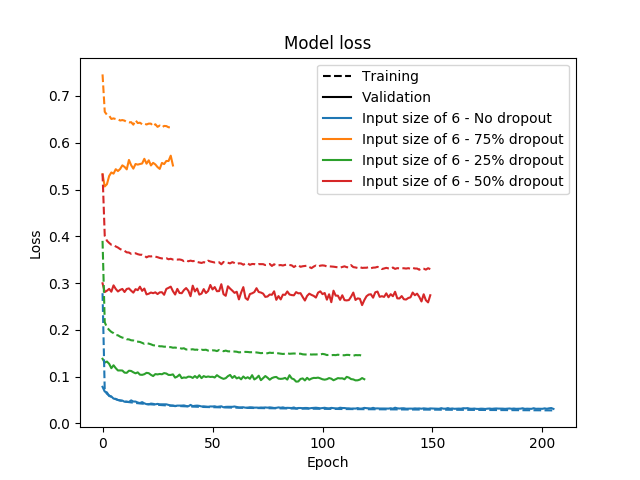
\includegraphics[width=0.5\textwidth]{drop11}
	\caption{Validation and training loss with each dropout factor, for input sizes of 6 samples.}
	\label{f:drop11}
\end{figure}

\begin{figure}[H]
	\centering
	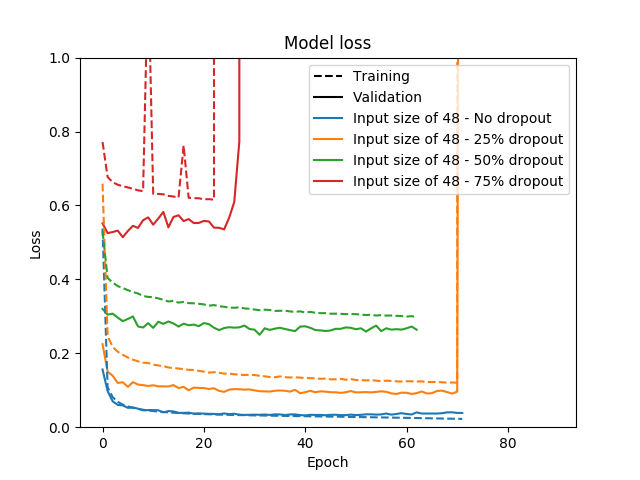
\includegraphics[width=0.5\textwidth]{drop12}
	\caption{Validation and training loss with each dropout factor, for input sizes of 48 samples.}
	\label{f:drop12}
\end{figure}

As we can see, on input sizes of 48 samples, applying a dropout factor makes gradients explode and loss takes very large values.

Gradient clipping prevents gradients from exploding. As we can see in table \ref{t:drop2} and figure \ref{f:drop2}, when all parameter gradients are clipped to a maximum norm of 1, we can successfully train our models while applying dropout.

\begin{table}[H]
	\centering
	\begin{tabular}{@{}ccccc@{}}
		\toprule
		&      & Training loss & Validation loss & Test loss \\ \midrule
		Input size of 48 & 0\%  & 0.02248       & 0.03962         & 0.03925   \\
		& 25\% & 0.11694       & 0.09555         & 0.09036   \\
		& 50\% & 0.28648       & 0.27258         & 0.25334   \\
		& 75\% & 0.59369       & 0.51817         & 0.48055   \\ \bottomrule
	\end{tabular}
	\caption{Results after testing different dropout factors and applying gradient clipping.}
	\label{t:drop2}
\end{table}

\begin{figure}[H]
	\centering
	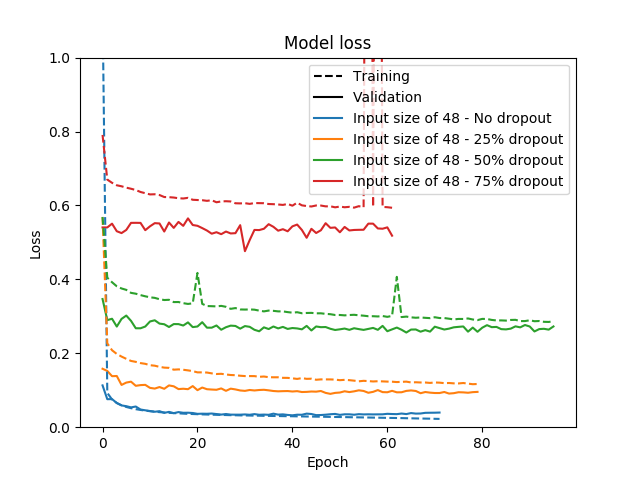
\includegraphics[width=0.5\textwidth]{drop2}
	\caption{Validation and training loss with each dropout factor, for input sizes of 48 samples, applying gradient clipping.}
	\label{f:drop2}
\end{figure}

Gradient clipping has demonstrated to be a good method for avoiding exploding gradients, hence we will conserve it in the following experiments. On the other hand, we found that applying dropout at the inter-layer connections and at the recurrent step does not improve the performance of our model at all; on the contrary, it gets much worse.

\subsection{Dropout II}

Taking into account that LSTMs solve the vanishing gradient problem using an internal state controlled by gates, it does not sound right to apply dropout over those gates. Probably the bad results obtained in the previous experiment can be prevented just applying dropout at the inter-layer connections but not at the recurrent step.

In this experiment we apply different dropout factors---25\%, 50\% and 75\%---after each LSTM layer.

Table \ref{t:drop3} shows the results obtained, while figures \ref{f:drop31} and \ref{f:drop32} show the evolution of the training and validation loss in each case.

\begin{table}[H]
	\centering
	\begin{tabular}{@{}ccccc@{}}
		\toprule
		&      & Training loss & Validation loss & Test loss \\ \midrule
		Input size of 6  & 0\%  & 0.02707       & 0.03102         & 0.03236   \\
		& 25\% & 0.03272       & 0.03107         & 0.03227   \\
		& 50\% & 0.04334       & 0.03215         & 0.03352   \\
		& 75\% & 0.06819       & 0.03617         & 0.03711   \\
		Input size of 48 & 0\%  & 0.02231       & 0.03864         & 0.04073   \\
		& 25\% & 0.03074       & 0.03451         & 0.03576   \\
		& 50\% & 0.03949       & 0.03425         & 0.03584   \\
		& 75\% & 0.06712       & 0.03815         & 0.03869   \\ \bottomrule
	\end{tabular}
	\caption{Results after testing different dropout factors, only between layers.}
	\label{t:drop3}
\end{table}

\begin{figure}[H]
	\centering
	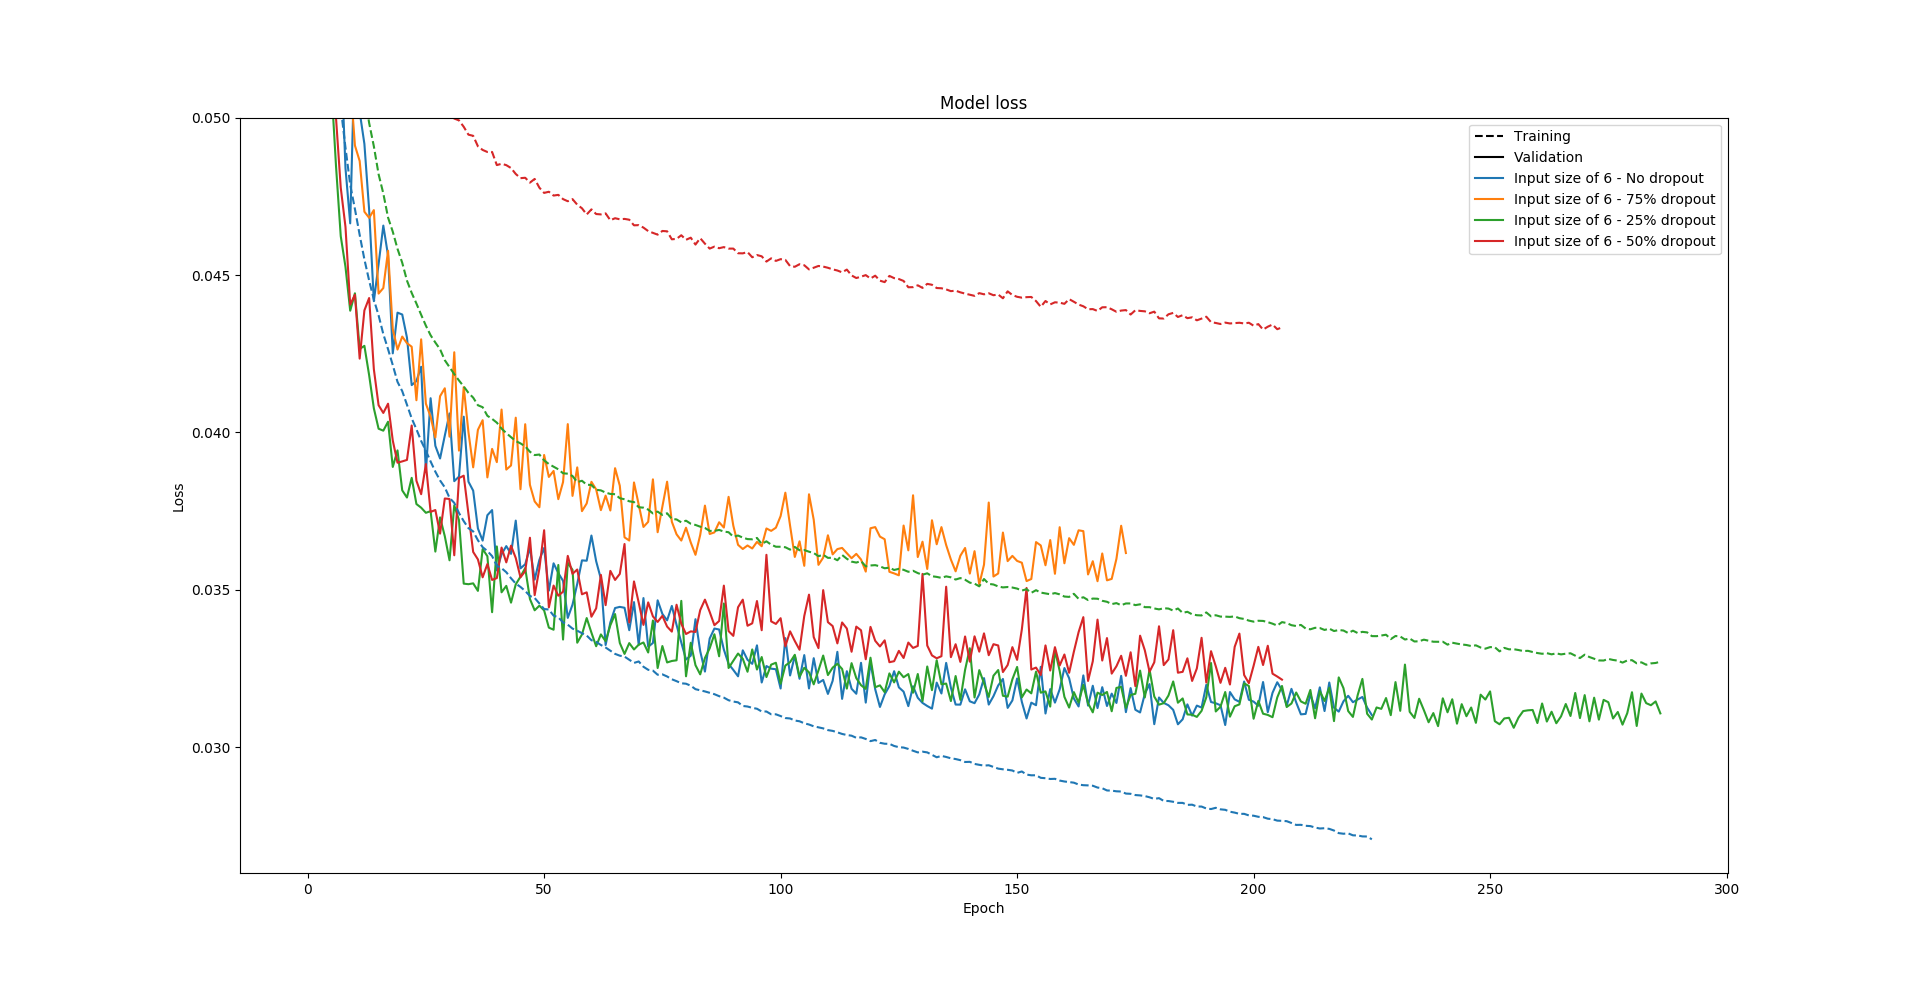
\includegraphics[width=\textwidth]{drop31}
	\caption{Validation and training loss with each dropout factor, for input sizes of 6 samples, only between layers.}
	\label{f:drop31}
\end{figure}

\begin{figure}[H]
	\centering
	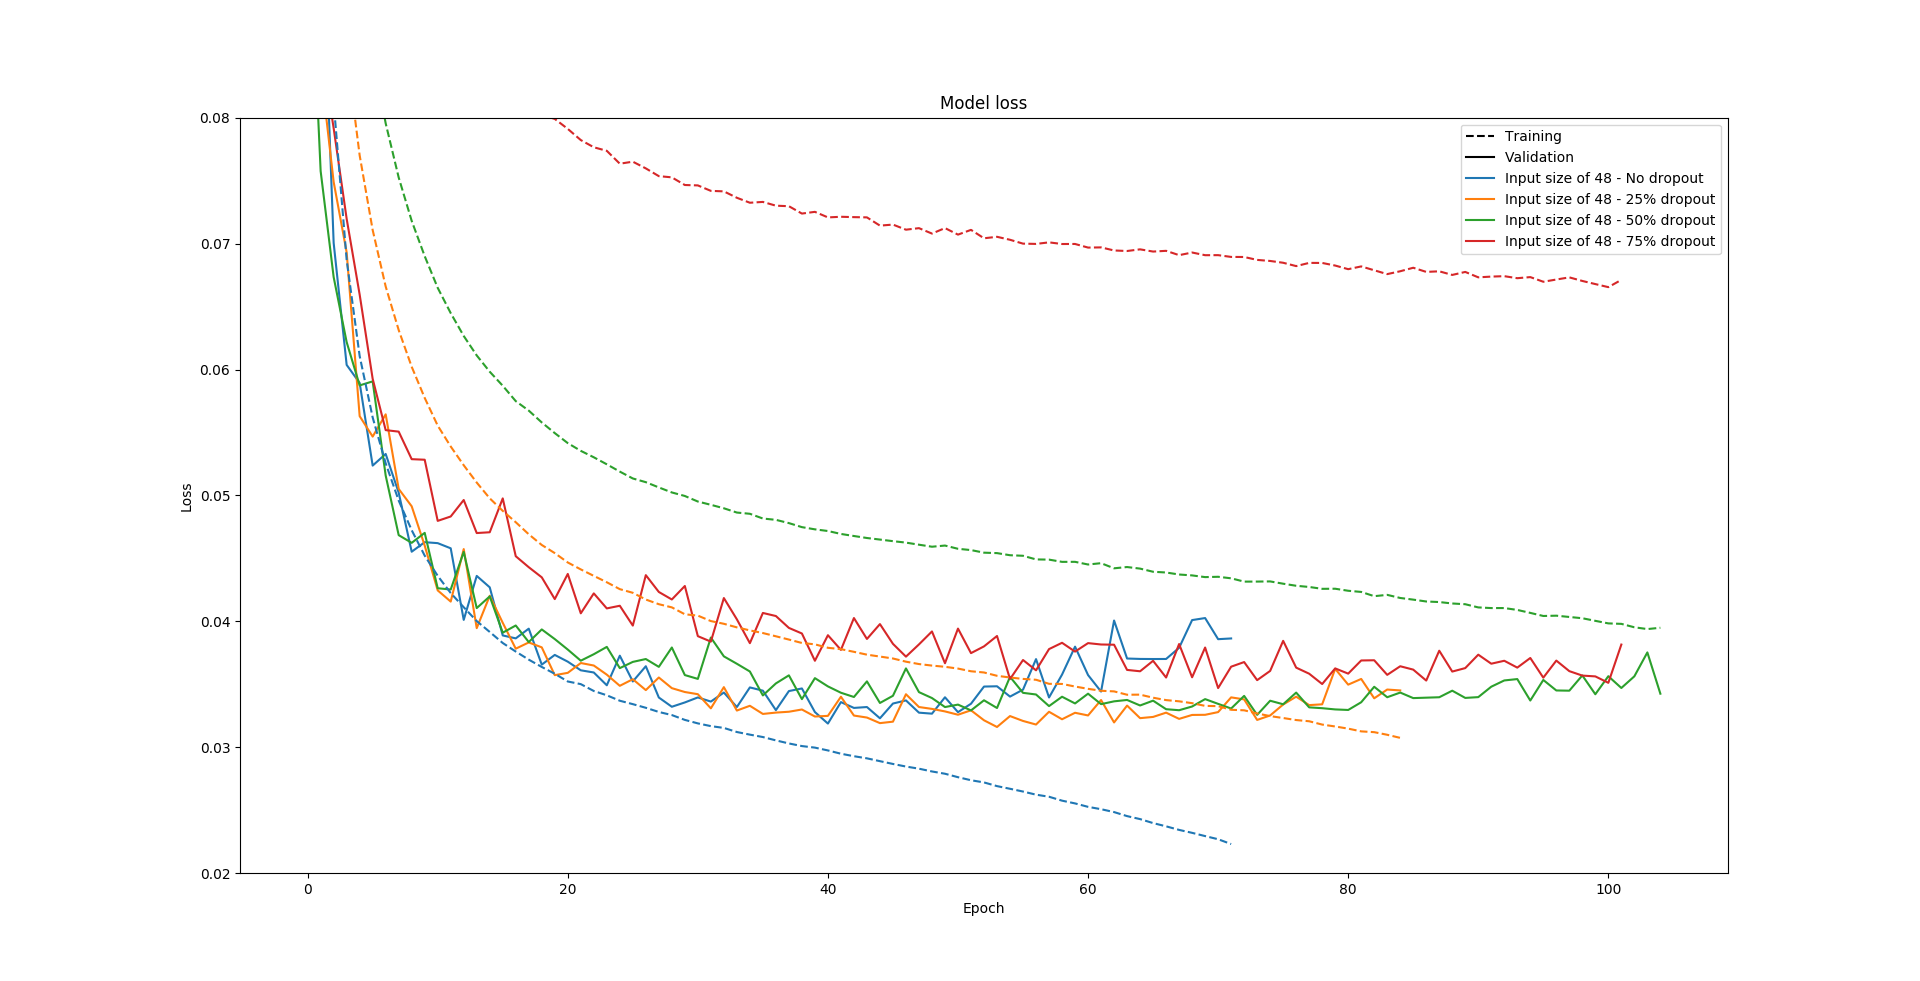
\includegraphics[width=\textwidth]{drop32}
	\caption{Validation and training loss with each dropout factor, for input sizes of 48 samples, only between layers.}
	\label{f:drop32}
\end{figure}

As we can see, dropout does make any considerable improvement when the input size is 6---probably because that model was not overfitting the training data---. However, when the input size is 48, we can see how a dropout of 25\% successfully reduces the gap between training and validation losses, obtaining an overall lower test error.

In any case, this model still has a worse performance than the model with an input size of 6.

\subsection{Sequential Architecture}

LSTM networks can learn the inherent data relations over intervals of time of \emph{any} length; however, in our current architecture, we train and test the model with short subsequences generated with a small sliding window.

Why are we doing that? Is it possible to train the LSTM model with all the data set expressed as a single huge sequence? By doing that, the LSTM network will learn whatever it finds relevant, and we will not arbitrarily decide its scope; the model will find the optimum one. It may happen that it finds data relations over very large intervals of time---maybe weeks---, improving the overall performance of the system.

In our current architecture, if we try to process our data set with a huge window size, we find a physical problem: there is not enough RAM.

When we process the data set, we go through $ N $ samples of $ V $ variables with a window size of $ W $, generating $ N - W $ vectors of $ V \cdot (W + 1) $ variables each. Since we train in batches of 1000, we are working with $ 1000 \cdot V \cdot (W + 1) $ variables simultaneously.

The memory used by this architecture is directly related to the size of sequences we use for training, making it not scalable for training with very large sequences of samples. We would need large amounts of RAM to exploit the true power of LSTM networks.

To overcome this obstacle, in this experiment we present a new architecture consisting in a sequence-to-sequence model that gives one prediction for each input we feed to it (i.e. when we feed a sequence of $ N $ inputs, the model gives $ N $ outputs). This new architecture completely discards the sliding window process and directly feeds the original measurements to the model, targeting the next 6 measurements of the data set for each given input.

This new model uses an option defined by Keras framework in their LSTM layer implementation\footnote{https://keras.io/layers/recurrent/\#lstm}, the argument ``stateful'': ``Boolean (default False). If True, the last state for each sample at index $ i $ in a batch will be used as initial state for the sample of index $ i $ in the following batch''.

In this new architecture each element of the training sequences pertain to different batches, hence the RAM used by the training process does not depend on the sequences size anymore. Now the required RAM only depends on the batch size we choose.

Our current data set, since it is sequentially sorted by time, is not compatible with this new training process and we must make a conversion first. This conversion consists in reordering the measurements in such a way that, for a data set of $ N $ samples and a batch size of $ B $, samples from $ s_1 $ to $ s_{\frac{N}{B}} $ end up being the 1st element of every batch, in sequential order; then samples from $ s_{\frac{N}{B}+1} $ to $ s_{\frac{N}{B}+\frac{N}{B}} $ end up being the 2nd element of every batch and so on.

As we can see, with this conversion we are actually generating $ B $ different training sequences. We can decide their size: with a batch size of 1 we train our model with a single sequence of 122,736 samples; with a batch size of 4 we train our model 4 sequences of size 30,684.

In this experiment we leave the batch size as 1000---so we train with input sequences of 122 samples---, in order to compare the results with the ones obtained in the previous experiments. We prefer to leave the same batch size because it directly affects to the model’s generalization, and results may vary.

In this experiment we also clip all parameter gradients to a maximum norm of 0.000000001---very, very small---and even with that we still suffer from exploding gradients, as it can be seen in figure \ref{f:architecture1}. In addition, this strict clipping slows the learning process: note that the gradients explode after after 2964 epochs---1 hour and 39 minutes in our hardware---and the training loss is not even below 0.8. We could test lower clipping norms but then the training process would take an unfeasible amount of time to finish.

\begin{figure}[H]
	\centering
	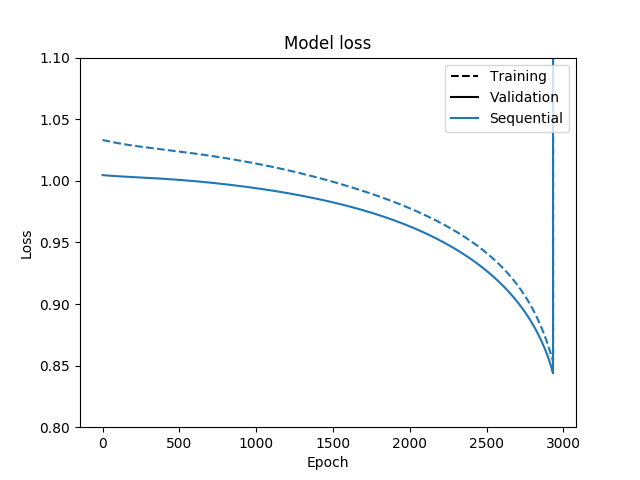
\includegraphics[width=0.5\textwidth]{architecture1}
	\caption{Exploding gradients when trying to train the sequential model.}
	\label{f:architecture1}
\end{figure}

Our gradients are exploding due to the usage of ReLU as activation function, since its range is $ [0, +\infty) $. If we replace it with the hyperbolic tangent---range $ (-1, 1) $---then we do not suffer this problem.

Table \ref{t:architecture2} shows the results obtained, while figure \ref{f:architecture2} shows the evolution of the training and validation loss in each case.

\begin{table}[H]
	\centering
	\begin{tabular}{@{}cccc@{}}
		\toprule
		& Training loss & Validation loss & Test loss \\ \midrule
		Sequential      & 0.03556       & 0.04878         & 0.05231   \\
		Input size of 6 & 0.02707       & 0.03102         & 0.03236   \\ \bottomrule
	\end{tabular}
	\caption{Results of the sliding window and the sequential model.}
	\label{t:architecture2}
\end{table}

\begin{figure}[H]
	\centering
	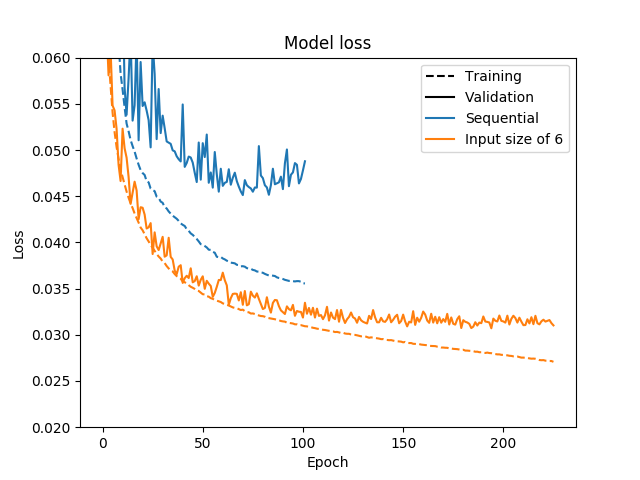
\includegraphics[width=0.5\textwidth]{architecture2}
	\caption{Validation and training loss of the sliding window and the sequential model.}
	\label{f:architecture2}
\end{figure}

This new architecture may be useful for problems where the model needs to recall information far from the past (e.g., stock price prediction or paragraph understanding) but it does not offer any advantage over our previous architecture based on a sliding window. From the previous experiments, we already had the suspicion that all the relevant information for making a good prediction relies on the very short past.

\section{Discussion of the Results}

In this practice we confirmed several expectations but also found cases where established methodologies have no effect in our context.

For example, regarding to the network topology, since two hidden layers can approximate any smooth variable relation to any accuracy, we found that our model experiments an improvement when we go from one hidden layer to two, and we do not experiment any improvement when using three. We could apply some deep learning techniques, such as layer-wise pre-training deep autoencoders with several layers, but it was out of the scope of this RNN practice.

Regarding to the activation function, as found by Clevert et al, 2016 and confirmed by us in the prior DL-MAI practice, we expected to speed up the training process and obtain a lesser error with ELUs. However, in this case, the change had no effect.

We have the suspicion that the cause behind this behavior relies on the data we are working with: easy to approximate, no matter the activation function, but with a constant underlaying noise, impossible to predict with the variables we have. With more variables, this noise can be reduced.

The rest of the activation functions we tested (logistic, hyperbolic tangent, softplus) obtain similar results than ReLU, confirming our suspicion.

Now, regarding to specific RNN properties, we found that larger window sizes do not improve the performance of the system, even when regularizing overfited models using dropout. Input sequences of 6 steps are enough to predict with the maximum accuracy we found the following 6. In fact, we also found that our alternative architecture consisting in a sequence-to-sequence model trained with very long sequences is not able to beat that mark neither.

Finally, regarding to regularization, we tested dropout and we found that in our case it is better not to apply it on the recursive step of the network, since the network performance is dramatically reduced. We suspect that dropout may interfere with the underlying state of the LSTM units, causing them to forget important information. If the model overfits, in our case, it is better to apply dropout between layers.

\section{Conclusion and Future Work}

In this practice we extended the experiments performed in the previous ``Guided Laboratory of the RNN Topic'', predicting more steps, trying more complex topologies and testing a sequence-to-sequence model.

We presented and followed a plan of experiments that lead us to confirm and discard several hypothesis, as explained in the prior section.

Due to the nature of the data set and the results of the performed experiments, in this practice we did not test different optimizers or regularization methods. Due to lack of time, we have not tried our model against other sites either, and we did not check the variance of our error. It is recommendable to perform n-fold cross-validation instead of a single test.

Finally, it would be also interesting to find a data set where our sequence-to-sequence architecture may obtain better results than the sliding window process. As previously said, this model can be useful on cases where long-term relations have special importance, such as on stock pricing prediction or text understanding.

\bibliography{bibfile}{}
\bibliographystyle{plain}

\end{document}
